%----------------------------------------------------------------------------------------
%	PRESENTATION SLIDES
%----------------------------------------------------------------------------------------


% to do :
% correct the task exercise
% add the end to the task csp extension problem


%------------------------------------------------
\section{IBM\cmark~ILOG CPLEX Optimization studio}
%------------------------------------------------

\begin{frame} \frametitle{Introduction to IBM\cmark ILOG CPLEX}
\pause		
CPLEX\rmark~Optimization Studio is composed of:\pause

\begin{itemize}[<+->]
\item IDE, an integrated development environment to develop and test models
\item OPL, the Optimization Programming Language, used to write mathematical models
\item CPLEX Optimizer engine, to find solutions to models that require mathematical programming techniques
\item CP Optimizer engine, to find solutions to models that require constraint programming techniques
\end{itemize}
	
\end{frame}


\begin{frame} \frametitle{Introduction to IBM\cmark~ILOG CPLEX}
\pause
Let's put the hands on the IDE for an interactive introduction, so follow the next steps:\pause

\begin{enumerate}[<+->]
\item Open the IDE
\item Create a workspace folder (use your universityID as name to avoid virtual machine problem)
\item Open the following template project for problem 1: \texttt{File/New/Example/IBM ILOG OPL Example/(quick search for) sched\_intro} 
\item Open the following template project for problem 2:
\texttt{File/New/Example/IBM ILOG OPL Example/(quick search for) sched\_jobshop}
\end{enumerate}

\end{frame}


\begin{frame} \frametitle{IDE overview}
\pause
To interact with the IDE (Eclipse friendly), \textbf{OPL Project} entities are used. These are objects composed by the following entities:\pause

\begin{itemize}[<+->]
	\item \textbf{Model} (of the problem) $\rightarrow$ \texttt{.mod} file
	\item \textbf{Input data} (instance of the problem) $\rightarrow$ \texttt{.dat} file
	\item \textbf{Settings} (of solving engines) $\rightarrow$ \texttt{.ops} file
	\item \textbf{Run Configuration} $\rightarrow$ wrapper to solve problem instance(s)
\end{itemize}

\end{frame}


\begin{frame} \frametitle{OPL}
\pause
A scheduling model has the same format as other models (.mod file) in OPL:\pause

\begin{itemize}[<+->]
	\item \textbf{Data structure} declarations
	\item \textbf{Decision variable} declarations 
	\item \textbf{Objective function} declarations
	\item \textbf{Constraint} declarations
\end{itemize}

\pause \medskip

OPL provides specialized \textbf{variables}, \textbf{constraints} and \textbf{keywords} designed for modelling scheduling problems.

\end{frame}


\begin{frame} \frametitle{Modelling scheduling problem}
\pause
OPL and CP Optimizer introduce a set of modeling features for applications that deal with scheduling over time.

\pause\medskip

In OPL with CP Optimizer, time points are represented as integers, but the possible very wide range of time points means that time is effectively continuous (\emph{time discretization}\only<3->{\footnote{In OPL, the unit of time represented by an interval decision variable is not defined.}}).

\pause\medskip

Most scheduling applications consist in scheduling over time a list of activities, tasks or operations that have a start and an end time. In CP Optimizer, this type of decision variable is captured by the notion of \textbf{interval variable}. 

\end{frame}


%------------------------------------------------
\section{Scheduling problems with IBM\cmark ILOG}
%------------------------------------------------

\begin{frame} \frametitle{Modelling scheduling problem}
\pause
Several types of constraints are expressed on and between interval variables:\pause

\begin{itemize}[<+->]
\item to limit the possible positions of an interval variable (forbidden start/end)
\item to specify precedence relations between two interval variables
\item to relate the position of an interval variable with one of a set of interval variables (spanning, synchronization, alternative)

\end{itemize}

\end{frame}


\begin{frame} \frametitle{Interval decision variables}
\pause
In OPL, tasks, such as the activities involved in scheduling problem, are modeled as intervals, represented by the \emph{decision variable type} \textbf{interval}.

\pause\medskip

Formally, an interval variable \textbf{a} is a variable whose domain is:\pause
\begin{equation*}
dom(a) \subseteq \{\perp\} \cup \{~[s,e)~|~s,e\in \mathcal{Z},~s\leq e\}.
\end{equation*} 

\pause\medskip

An interval variable is said to be \textbf{fixed} if its domain is reduced to a singleton; that is, if \textbf{\texttt{\underline{a}}} denotes a fixed interval variable:\pause
\begin{itemize}[<+->]
\item Interval is absent:  \textbf{\texttt{\underline{a}}} $ = \{\perp\}$
\item Interval is present: \textbf{\texttt{\underline{a}}} $ = [s,e)$

\end{itemize}

\end{frame}


\begin{frame} \frametitle{Interval decision variables}
\pause
The semantics of constraints defined over interval variables is described by the properties that fixed intervals must have in order the constraint to be true.

\pause\medskip

If a \emph{fixed} interval \textbf{\texttt{\underline{a}}} is present and such that \textbf{\texttt{\underline{a}}} $= [s,e)$ , we will denote:\pause
\begin{itemize}[<+->]
\item \textbf{\texttt{s(\underline{a})}} its integer \emph{start} value $s$
\item \textbf{\texttt{e(\underline{a})}} its integer \emph{end} value $e$
\item \textbf{\texttt{l(\underline{a})}} its positive integer \emph{length} defined as \texttt{\textbf{e(\underline{a})} - \textbf{s(\underline{a})}} 
\item \textbf{\texttt{x(\underline{a})}} the presence that will be equal to $1$
\end{itemize}

\pause\medskip

For an \emph{absent} interval, $\textbf{\texttt{x(\underline{a})}} = 0$ and \textbf{\texttt{s(\underline{a})}},\textbf{\texttt{e(\underline{a})}} and \textbf{\texttt{l(\underline{a})}} are undefined.

\end{frame}

\begin{frame} \frametitle{Interval decision variables (syntax)}
\pause
General syntax for declaring interval decision variable:

\pause\medskip

\begin{equation*}
\texttt{dvar interval <taskName><switches>;} 
\end{equation*}

\pause\medskip

where \textbf{\texttt{<switches>}} represents one or more different modifying conditions to be applied to the interval. 

\end{frame}

\begin{frame} \frametitle{Interval decision variables (switches)}
\pause
\textbf{Time window} setting for a interval decision variables:\pause
\begin{equation*}
\texttt{dvar interval masonry in 0..20;} 
\end{equation*}

\pause\medskip

A task may have a fixed size, but processing may be suspended during a break, so that the length is greater than the size.

\pause\medskip

\textbf{Size} switch provides different length to an interval.
\pause
\begin{equation*}
\texttt{dvar interval windows size 5 in 0..7;} 
\end{equation*}
\pause
In the example, the \emph{windows} task may take $5$ days to install (interval's size), but if work stops over a two-day weekend, the length of the \emph{windows} interval decision variable would be 7.

\end{frame}


\begin{frame} \frametitle{Interval decision variables (switches)}

\textbf{Optional} interval decision variables declaration:\pause
\begin{equation*}
\texttt{dvar interval garden optional;} 
\end{equation*}
\pause
An optional interval may or may not be present in the solution.

\end{frame}


\begin{frame} \frametitle{30 seconds question}

What does it means this variable declaration:\pause
\begin{equation*}
\texttt{dvar interval garden optional in 20..32 size 5;} 
\end{equation*}
\pause
\textbf{Solution:} 
\pause
\begin{itemize}[<+->]
\item is an interval decision variable 
\item is optional
\item has size 5
\item its time window starts at 20 and end at 32
\item with length?
\end{itemize}

\end{frame}

\begin{frame} \frametitle{Precedence constraints on intervals}

Precedence constraints are common scheduling constraints used to restrict the relative position of interval variables in a solution.

\pause\medskip

These constraints are used to specify when one interval variable must start or end with respect to the start or end time of another interval.\pause
\begin{itemize}[<+->]
\item \textbf{\texttt{(start|end)Before(Start|End)}}
\item \textbf{\texttt{(start|end)At(Start|End)}}
\end{itemize}

\end{frame}

\begin{frame} \frametitle{Precedence constraints on intervals (syntax)}

$\textbf{\texttt{endBeforeStart (a,b[,z]);}}$

\pause\medskip

Express the end of a given time interval \textbf{\texttt{a}} (modified by an optional time value \textbf{\texttt{z}}) is less than or equal to the start of a given time interval \textbf{\texttt{b}}:

\pause\medskip 

$\textbf{\texttt{e(a) + z $\leq$ s(b)}}$

\pause\medskip

Where:\pause
\begin{itemize}[<+->]
	\item \textbf{\texttt{s(x)}} is the starting time of the interval \textbf{\texttt{x}}
	\item \textbf{\texttt{e(x)}} is the ending time of the interval \textbf{\texttt{x}}
\end{itemize}

\end{frame}

\begin{frame} \frametitle{Precedence constraints on intervals (semantic)}

Let \textbf{\texttt{TC(\underline{a},\underline{b},z)}} the precedence relation on a pair of fixed intervals \textbf{\texttt{\underline{a},\underline{b}}} and \textbf{\texttt{z}} a given value, the following table express its semantic:

\pause\medskip

\begin{table}[h]
%\caption{Average objectives functions values reached in the largest instance class (250 jobs and 20 machines).}
%\label{tab:250_20}
\centering
%	\resizebox{\columnwidth}{!}{
\begin{tabular}{|l|l|}
\hline
Expression									 			& Semantics \\ \hline
\bfttt{startBeforeStart(\underline{a},\underline{b},z)}	& $\bfttt{x(\underline{a})} \wedge  \bfttt{x(\underline{b})} \Rightarrow \bfttt{s(\underline{a})} + z \leq \bfttt{s(\underline{b})}$  \\ \hline
\bfttt{startBeforeEnd(\underline{a},\underline{b},z)}	& $\bfttt{x(\underline{a})} \wedge  \bfttt{x(\underline{b})} \Rightarrow \bfttt{s(\underline{a})} + z \leq \bfttt{e(\underline{b})}$  \\ \hline
\bfttt{endBeforeStart(\underline{a},\underline{b},z)}	& $\bfttt{x(\underline{a})} \wedge  \bfttt{x(\underline{b})} \Rightarrow \bfttt{e(\underline{a})} + z \leq \bfttt{s(\underline{b})}$  \\ \hline
\bfttt{endBeforeEnd(\underline{a},\underline{b},z)}		& $\bfttt{x(\underline{a})} \wedge  \bfttt{x(\underline{b})} \Rightarrow \bfttt{e(\underline{a})} + z \leq \bfttt{e(\underline{b})}$  \\ \hline
\bfttt{startAtStart(\underline{a},\underline{b},z)}		& $\bfttt{x(\underline{a})} \wedge  \bfttt{x(\underline{b})} \Rightarrow \bfttt{s(\underline{a})} + z = \bfttt{s(\underline{b})}$  \\ \hline
\bfttt{startAtEnd(\underline{a},\underline{b},z)}		& $\bfttt{x(\underline{a})} \wedge  \bfttt{x(\underline{b})} \Rightarrow \bfttt{s(\underline{a})} + z = \bfttt{e(\underline{b})}$  \\ \hline
\bfttt{endAtStart(\underline{a},\underline{b},z)}		& $\bfttt{x(\underline{a})} \wedge  \bfttt{x(\underline{b})} \Rightarrow \bfttt{e(\underline{a})} + z = \bfttt{s(\underline{b})}$  \\ \hline
\bfttt{endAtEnd(\underline{a},\underline{b},z)}			& $\bfttt{x(\underline{a})} \wedge  \bfttt{x(\underline{b})} \Rightarrow \bfttt{e(\underline{a})} + z = \bfttt{e(\underline{b})}$  \\ \hline
\end{tabular}
%	}
\end{table}

\end{frame}


\begin{frame} \frametitle{30 seconds question}

How to specify that \bfttt{task1} have to finish \bfttt{10} time unit before \bfttt{task2} start?

\pause\medskip~\medskip

\textbf{Solution:} 
\begin{equation*}
\texttt{endBeforeStart(task1, task2, 10);} 
\end{equation*}

\end{frame}


%------------------------------------------------
\section{Practical exercise}
%------------------------------------------------

%------------------------------------------------
\subsection{Schedule building task (CSP)}
%------------------------------------------------


\begin{frame} \frametitle{Problem description}

This is a basic problem that involves building a house. Different tasks have to be scheduled and some of them have to take place before others. 

\pause\medskip

Tasks: \bfttt{masonry, carpentry, plumbing, ceiling, roofing, painting, windows, facade, garden, moving.}

\pause\medskip 

Precedence constraints:\pause
\begin{itemize}[<+->]
	\item \bfttt{masonry $\leq$ carpentry, plumbing, ceiling}
	\item \bfttt{carpentry $\leq$ roofing}
	\item \bfttt{ceiling $\leq$ painting}
	\item \bfttt{roofing $\leq$ windows, facade, garden}
	\item \bfttt{plumbing $\leq$ facade, garden}
	\item \bfttt{moving $\geq$  painting, windows, facade, garden}	
\end{itemize}

\pause\medskip 

Run a configuration to find a solution!

\end{frame}

\begin{frame} \frametitle{Problem extension}

To extend the problem you can follow this step:\pause
\begin{itemize}[<+->]
	\item Create a new \textbf{model} to represent the extended problem (right-click on the project folder/New/Model)
	\item Create a new \textbf{run configuration} (right-click on the project folder/New/Run Configuration)
	\item modify the \bfttt{.mod} file and add it to the new \textbf{run configuration}
\end{itemize}

\end{frame}

\begin{frame} \frametitle{Problem extension}
\pause
Due to an unexpected, tasks chnaged and new ones are added, in details:\pause
\begin{itemize}[<+->]
	\item \bfttt{moving} double its execution time and be the last task
	\item New tasks: \bfttt{dependence (15), swimmingPool (10), gazebo (5), dogHouse (5)}
	\item \bfttt{dependance} has to finish 5 time unit before the (start of) \bfttt{garden} 
	\item \bfttt{swimmingPool} has to start after (end of) \bfttt{facade} and finish at least 7 time unit before the (start of) \bfttt{garden}
	\item \bfttt{garden} has to finish before (start of) \bfttt{gazebo} and (start of) \bfttt{dogHouse}
\end{itemize}

\pause\medskip

Model the new problem and run a configuration. Good work!

\end{frame}

\begin{frame} \frametitle{Problem extension assessment}
\pause
Exercise:\pause
\begin{enumerate}[<+->]
	\item Inspect the new code and focus your attention on the advanced constructs
	\item Run a configuration and inspect the decision variables (toogle between the visualization mode)
	\item \label{ex:makespan} find the makespan value
	\item \label{ex:analysis} inspection the scheduling solution, identify and write down the first and last task done in each machine (ex. machine $m$ execute as first/last task $ij$)
	\item find the task responsible for the makespan, half its processing time (rounded by ceiling) and run a new configuration. Do exercises \ref{ex:makespan} and \ref{ex:analysis} over the new solution.
\end{enumerate}

\pause \medskip

You have 10 minutes!

\end{frame}



%------------------------------------------------
\subsection{Advanced scheduling constructs}
%------------------------------------------------

\begin{frame} \frametitle{Expression on interval variables}

Integer expressions are available to access or evaluate different attributes of an interval variable. 

\pause\medskip

These expressions can be used, for example, to define a term for the cost function or to connect interval variables to integer and floating point expressions.

\pause\medskip

The integer expressions are \bfttt{startOf, endOf, lengthOf, sizeOf} and they provide access to the different attributes of an interval variable.

\pause\medskip

Special care must be taken for optional intervals, as an integer value dval must be specified which represents the value of the expression when the interval is absent. If this value is omitted, it is supposed to be 0. 

\end{frame}

\begin{frame} \frametitle{Expression on interval variables (semantic)}

Let \bfttt{\underline{a}} a fixed interval variable. The semantics of these expressions is shown below:

\pause\medskip

\begin{table}[h]
%\caption{Average objectives functions values reached in the largest instance class (250 jobs and 20 machines).}
%\label{tab:250_20}
\centering
%	\resizebox{\columnwidth}{!}{
\begin{tabular}{|l|l|}
\hline
Expression		 						& Semantics \\ \hline
\bfttt{startOf(\underline{a},dval)}		& $
\begin{cases} 
\bfttt{s(\underline{a})}	& \text{if \bfttt{x(\underline{a})}}\\
\bfttt{dval}		   		& \text{otherwise }
\end{cases}
$ \\ \hline
\bfttt{endOf(\underline{a},dval)}		& $
\begin{cases} 
\bfttt{e(\underline{a})}	& \text{if \bfttt{x(\underline{a})}}\\
\bfttt{dval}		   		& \text{otherwise }
\end{cases}
$ \\ \hline
\bfttt{lengthOf(\underline{a},dval)}		& $
\begin{cases} 
\bfttt{l(\underline{a})}	& \text{if \bfttt{x(\underline{a})}}\\
\bfttt{dval}		   		& \text{otherwise }
\end{cases}
$ \\ \hline
\bfttt{sizeOf(\underline{a},dval)}		& $
\begin{cases} 
\bfttt{size(\underline{a})}	& \text{if \bfttt{x(\underline{a})}}\\
\bfttt{dval}		   		& \text{otherwise }
\end{cases}
$ \\ \hline
\end{tabular}
%	}
\end{table}

\end{frame}


\begin{frame} \frametitle{Sequence decision variables}

An \textbf{interval sequence variable} is defined on a set of interval variables $\mathcal{A}$. Informally speaking, the value of an interval sequence variable represents a total ordering of the interval variables of $\mathcal{A}$. Note that any absent interval variables are not considered in the ordering.
 
\pause\medskip

More formally, an interval sequence variable \bfttt{p} on a set interval variables $\mathcal{A}$ represents a decision variable whose possible values are all the permutations of the intervals of $\mathcal{A}$.

\pause\medskip

Note that the sequence alone does not enforce any constraint on the relative position of intervals end-points. For instance, an interval variable \bfttt{a} could be sequenced before an interval variable \bfttt{b} in a sequence \bfttt{p} without any impact on the relative position between the start/end points of \bfttt{a} and \bfttt{b} (a could still be fixed to start after the end of b).

\end{frame}

\note{
Clarify: For instance, an interval variable a could be sequenced before an interval variable b in a sequence p without any impact on the relative position between the start/end points of a and b (a could still be fixed to start after the end of b). This is because different semantics can be used to define how a sequence constrains the positions of intervals.
	
}


\begin{frame} \frametitle{Sequence decision variables (syntax)}
\pause

\bfttt{dvar sequence p in A [types T];}\\
Where:\\
\bfttt{dvar interval A[];}\\
\bfttt{int T[];}\\

\pause\medskip

A sequence variable represents a total order over a set of interval variables. If a sequence \bfttt{p} is defined over a set of interval variables \bm{$A=\{a_1,a_2,a_3,a_4\}$}, a value for this sequence can be: \bm{$(a_3,a_1,a_4,a_2)$}.

\pause\medskip

A non-negative integer (the type, i.e. \bfttt{T}) can be associated with each interval variable in the sequence. This integer is used by some constraints on the sequence. Basically, from the perspective of the constraints on the sequence variable, intervals with the same type share some common features.

\pause\medskip

Note that absent interval variables are not considered in the ordering

\end{frame}

\note{
Clarify: For instance, an interval variable a could be sequenced before an interval variable b in a sequence p without any impact on the relative position between the start/end points of a and b (a could still be fixed to start after the end of b). This is because different semantics can be used to define how a sequence constrains the positions of intervals.

}


\begin{frame} \frametitle{Constraint on sequence variables}
\pause

The following constraints are available on sequence variables:\pause
\begin{itemize}[<+->]
\item \bfttt{first(p,a)} states that if interval \bfttt{a} is present, then it will be the \textbf{first} interval of sequence \bfttt{p}.
\item \bfttt{last(p,a)} states that if interval \bfttt{a} is present, then it will be the \textbf{last} interval of sequence \bfttt{p}.
\item \bfttt{before(p,a,b)} states that if both interval \bfttt{a} and \textbf{b} are present, then \bfttt{a} will appear \textbf{before} \bfttt{b} in sequence \bfttt{p}.
\item \bfttt{prev(p,a,b)} states that if both interval \bfttt{a} and \textbf{b} are present, then \bfttt{a} will appear \textbf{just before} \bfttt{b} and no other intervals will be sequenced between \bfttt{a} and \textbf{b} in sequence \bfttt{p}.
\end{itemize}

\end{frame}


\begin{frame} \frametitle{Constraint on sequence variables (semantic)}

The formal semantics of these basic constraints is shown in the below::

\pause\medskip

\begin{table}[h]
%\caption{Average objectives functions values reached in the largest instance class (250 jobs and 20 machines).}
%\label{tab:250_20}
\centering
\begin{tabular}{|l|l|}
\hline
Expression							& Semantics \\ \hline
\bfttt{first($\pi$,\underline{a})}	& $\bfttt{x(\underline{a})} \Rightarrow (\bfttt{$\pi$(\underline{a}) = 1})$  \\ \hline
\bfttt{last($\pi$,\underline{a})}	& $\bfttt{x(\underline{a})} \Rightarrow (\bfttt{$\pi$(\underline{a}) = length(s)})$  \\ \hline
\bfttt{before($\pi$,\underline{a},\underline{b})}	&  $(\bfttt{x(\underline{a})} \wedge \bfttt{x(\underline{b})}) \Rightarrow (\bfttt{$\pi$(\underline{a})} \leq \bfttt{$\pi$(\underline{b})})$ \\ \hline
\bfttt{prev($\pi$,\underline{a},\underline{b})}	&  $(\bfttt{x(\underline{a})} \wedge \bfttt{x(\underline{b})}) \Rightarrow (\bfttt{$\pi$(\underline{b})} = \bfttt{$\pi$(\underline{a}) + 1})$ \\ \hline
\end{tabular}
\end{table}

Where \bfttt{$\pi$(\underline{a})} is the positional value of interval variable \bfttt{\underline{a}} over the sequence variable $\pi$.

\end{frame}


\begin{frame} \frametitle{No Overlap constraint}

The \textbf{no overlap constraint} on an interval sequence variable \bfttt{p} states that the sequence defines a chain of non-overlapping intervals, any interval in the chain being constrained to end before the start of the next interval in the chain. This constraint is typically useful for modelling disjunctive resources.

More formally, the condition for a permutation value $\pi$ of sequence \bfttt{p} to satisfy the \bfttt{noOverlap} constraints is defined as:


\pause

\begin{align*}
& \bfttt{noOverlap($\pi$)} \Leftrightarrow \\
& \forall \bfttt{\underline{a},\underline{b}} \in \underline{A}, \quad \neg \bfttt{x(\underline{a})} \vee \bfttt{x(\underline{b})} \vee ((\bfttt{$\pi$(\underline{a})} < \bfttt{$\pi$(\underline{b})}) \Leftrightarrow (\bfttt{e(\underline{a})} \leq \bfttt{s(\underline{b})}))
\end{align*}

\end{frame}


%------------------------------------------------
\subsection{Classic job-shop scheduling problem (COP)}
%------------------------------------------------

\begin{frame} \frametitle{Job-shop scheduling problem (JSP)}
\pause
General information:\pause
\begin{itemize}[<+->]
\item Combinatorial optimization problem in which ideal jobs are assigned to resources at particular times
\item benchmark for exact and approximated techniques
\item widely studied in literature 
\end{itemize}

\pause\medskip

\begin{figure}
\centering
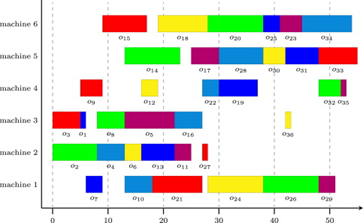
\includegraphics[width=.5\columnwidth]{jobshop}
%\caption{Interaction sequence to solve the distributed scheduling problem}
\end{figure}




\end{frame}

\begin{frame} \frametitle{Job-shop scheduling problem (JSP)}
\pause
Informal description:\pause
\begin{itemize}[<+->]
\item n jobs, each one composed of a set of operations/tasks
\item m machines, where tasks have to be processed
\item each task has to be processed only on one machine with a predefined processing time and order between tasks
\item usual objective is to minimize the makespan: ending time of the last task
\end{itemize}

\medskip

\begin{figure}
\centering
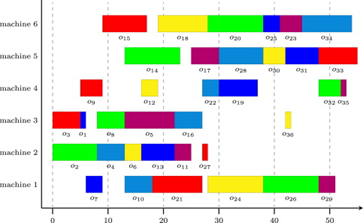
\includegraphics[width=.5\columnwidth]{jobshop}
%\caption{Interaction sequence to solve the distributed scheduling problem}
\end{figure}

\end{frame}

\begin{frame} \frametitle{Job-shop scheduling problem}
\pause
Problem data:
\begin{itemize}[<+->]
\item $p_{ij}$ is the processing time for task $i$ of job $j$ 
\end{itemize}

\medskip

Variables:
\begin{itemize}[<+->]
\item $st_{ij}$ starting time for task $i$ of job $j$ 
\end{itemize}


\medskip

Constraints:
\begin{itemize}[<+->]
\item Sequential: $st_{ij} + p_{ij} \leq st_{i(j+1)}$
\item Capacity: $st_{ij} + p_{ij} \leq st_{kl} \vee st_{kl} + p_{kl} \leq st_{ij}$
\item No-preemption: $c_{ij} = st_{ij} + p_{ij}$
\end{itemize}

\medskip

\begin{figure}
	\centering
	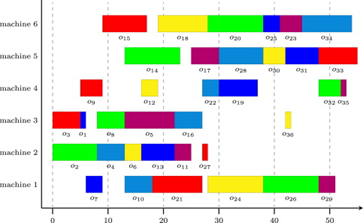
\includegraphics[width=.5\columnwidth]{jobshop}
	%\caption{Interaction sequence to solve the distributed scheduling problem}
\end{figure}

\end{frame}

\begin{frame} \frametitle{Job-shop scheduling problem (JSP)}
\pause
Solution:\pause
\begin{itemize}[<+->]
\item Build an order over the time for all the tasks, so that all constraints on each machine are satisfied
\end{itemize}

\medskip

Objective:
\begin{itemize}[<+->]
\item Minimize the makespan: $\operatorname*{min} C_{max} = \operatorname*{min}~\operatorname*{max}_{j}  C_{ij}$
\item Minimize the total flow time: $\operatorname*{min}~C_{sum} = \operatorname*{min} \sum C_{i}$
\end{itemize}


\medskip

\begin{figure}
	\centering
	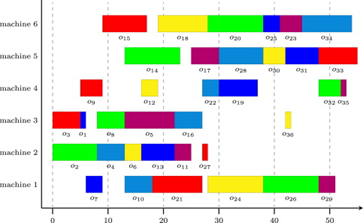
\includegraphics[width=.5\columnwidth]{jobshop}
	%\caption{Interaction sequence to solve the distributed scheduling problem}
\end{figure}

\end{frame}


\begin{frame} \frametitle{Job-shop scheduling problem (JSP)}
\pause
How to solve a Job-shop scheduling problem (JSP):\pause
\begin{itemize}[<+->]
\item Complete search
\item Constraint programming
\item Meteheuristic
\item Commercial solver
\item \dots
\end{itemize}


\end{frame}

%------------------------------------------------
\subsection{Job-shop scheduling problem scenario}
%------------------------------------------------

\begin{frame} \frametitle{JSP scenario}
\pause
In the opened project (\texttt{sched\_jobshop}) you will find new file types:\pause
\begin{itemize}[<+->]
\item A problem instance data file (\texttt{.dat} file)
\item A setting file (\texttt{.ops} file)
\end{itemize}

\pause \medskip

This files are needed any time you have to solve the model (the setting file is optional, if not present in a run configuration, default values for the solver will be used).

\end{frame}


\begin{frame} \frametitle{JSP scenario}
\pause
Exercise:\pause
\begin{enumerate}[<+->]
\item Inspect the new code and focus your attention on the advanced constructs
\item Run a configuration and inspect the decision variables (toogle between the visualization mode)
\item \label{ex:makespan} find the makespan value
\item \label{ex:analysis} inspection the scheduling solution, identify and write down the first and last task done in each machine (ex. machine $m$ execute as first/last task $ij$)
\item find the task responsible for the makespan, half its processing time (rounded by ceiling) and run a new configuration. Do exercises \ref{ex:makespan} and \ref{ex:analysis} over the new solution.
\end{enumerate}

\pause \medskip

You have 10 minutes!

\end{frame}

\begin{frame} \frametitle{JSP scenario}
\pause
From the \texttt{sched\_jobshop} template, model the \emph{readers and newspapers} problem.

\pause \medskip

There are 3 newspapers $(N_1, N_2, N_3)$ and 4 readers $(R_1, R_2, R_3, R_4)$, who wish to read newspapers in the same order $(N_1 < N_2 < N_3)$. Each reader has a different \emph{reading time} depending on the newspaper according to the following table:

\pause \medskip

\begin{table}
\centering
\begin{tabular}{|l|c|c|c|c|}
\hline
		& $N_1$	& $N_2$	& $N_3$	\\ \hline
$R_1$	& 5		& 10	& 2		\\ \hline
$R_2$	& 2		& 6		& 5		\\ \hline
$R_3$	& 10	& 15	& 15	\\ \hline
$R_4$	& 3		& 5		& 5		\\ \hline
\end{tabular}

\end{table}

\pause

\begin{center}
Model it in the OPL language, run a suitable configuration and repeat the previous exercises!
\end{center}

\begin{center}
You have 10 minutes time! 
\end{center}


\end{frame}


\begin{frame} \frametitle{JSP scenario advanced}
\pause
From the previous exercise we extend the \emph{readers and newspapers} problem introducing ready time and due date for the newspapers.

\pause \medskip

Same scenario as before, but this time each reader has two new constraints: a \emph{ready time} (the first moment when he can start to read) and a \emph{due date} (the time before all the newspapers have to been read). The \emph{ready time} and \emph{due date} are according to the following table:

\pause \medskip

\begin{table}
\centering
\begin{tabular}{|l|c|c|c|c|c|c|}
\hline
		& Ready	& $P_1$	& $P_2$	& $P_3$	& DueDate	\\ \hline
$L_1$	& 0		& 5		& 10	& 2		& 30		\\ \hline
$L_2$	& 0		& 2		& 6		& 5		& 20		\\ \hline
$L_3$	& 0		& 10	& 15	& 15	& 60		\\ \hline
$L_4$	& 0		& 3		& 5		& 5		& 15		\\ \hline
\end{tabular}
	
\end{table}

\pause

\begin{center}
	Model it in the OPL language, run a suitable configuration and repeat the previous exercises!
\end{center}

\begin{center}
	You have time till the lesson end, plus Easter holiday! 
\end{center}


\end{frame}


%------------------------------------------------
\section{Useful links and references}
%------------------------------------------------

\begin{frame} \frametitle{OPL references}

Official software download \href{https://developer.ibm.com/academic/resources/data-analytics}{\underline{\textcolor{blue}{link}}} and official web references:\footnote{Click to be redirected to the web page}

\begin{itemize}
\item \href{http://www.ibm.com/support/knowledgecenter/SSSA5P_12.7.1/ilog.odms.ide.help/OPL_Studio/gsoplide/topics/opl_ide_gettingstarted_TOC.html?lang=en}{Getting started with the IDE}
\item \href{http://www.ibm.com/support/knowledgecenter/SSSA5P_12.7.1/ilog.odms.ide.help/OPL_Studio/opllangref/topics/opl_langref_datastructures.html?lang=en}{OPL Data structure}
\begin{itemize}
\item \href{http://www.ibm.com/support/knowledgecenter/SSSA5P_12.7.1/ilog.odms.ide.help/OPL_Studio/opllangref/topics/opl_langref_data_init_arrays.html?lang=en}{Generic arrays}
\item \href{http://www.ibm.com/support/knowledgecenter/SSSA5P_12.7.1/ilog.odms.ide.help/OPL_Studio/opllangref/topics/opl_langref_scheduling_interval.html?lang=en}{Interval variables}
\item \href{http://www.ibm.com/support/knowledgecenter/SSSA5P_12.7.1/ilog.odms.ide.help/OPL_Studio/opllangref/topics/opl_langref_scheduling_precedence.html?lang=en}{Precedence constraints}
\item \href{http://www.ibm.com/support/knowledgecenter/SSSA5P_12.7.1/ilog.odms.ide.help/OPL_Studio/opllangref/topics/opl_langref_scheduling_expressions.html?lang=en}{Expressions on intervals}
\item \href{http://www.ibm.com/support/knowledgecenter/SSSA5P_12.7.1/ilog.odms.ide.help/OPL_Studio/opllangref/topics/opl_langref_scheduling_sequence.html?lang=en}{Interval sequence variables}
\end{itemize}
\item \href{http://www.ibm.com/support/knowledgecenter/SSSA5P_12.7.1/ilog.odms.ide.help/OPL_Studio/scheduling_gs/topics/opl_gs_scheduling.html?lang=en}{Getting started with Scheduling}
\item \href{http://www.ibm.com/support/knowledgecenter/SSSA5P_12.7.1/ilog.odms.ide.help/OPL_Studio/opllangref/topics/opl_langref_scheduling.html?lang=en}{Scheduling with CP}
\end{itemize}
 
\end{frame}


\begin{frame} \frametitle{Scheduling references}

\begin{itemize}
\item{}[J. Y-T. Leung] Handbook of Scheduling: Algorithms, Models, and Performance Analysis. 
\item{}[M. L. Pinedo] Scheduling: Theory, Algorithms, and Systems. 
\end{itemize}

\end{frame}


\begin{comment}

\begin{frame}[t, allowframebreaks] \frametitle{References}
\bibliographystyle{amsalpha}
\bibliography{refs/references}
\end{frame}


\end{comment}



%------------------------------------------------

\begin{frame} \frametitle{~}
\Huge{\centerline{Thank you for your attention}}

\medskip~\medskip



\footnotesize To evaluate and improve actual and future delivering quality, you are gently asked to fill in this 5 minutes \href{https://docs.google.com/forms/d/e/1FAIpQLSfwxSb55IaeGEbYmbwQi0rnjXxNqUQVUr_sxtMGVZk4cPvWMw/viewform?usp=sf_link}{\textcolor{blue}{\underline{form}}}\footnote{DL 15 of May 2017}


\end{frame}
